% Created 2021-10-18 Mon 07:48
% Intended LaTeX compiler: pdflatex
\documentclass[presentation,aspectratio=169, usenames, dvipsnames]{beamer}
\usepackage[utf8]{inputenc}
\usepackage[T1]{fontenc}
\usepackage{graphicx}
\usepackage{grffile}
\usepackage{longtable}
\usepackage{wrapfig}
\usepackage{rotating}
\usepackage[normalem]{ulem}
\usepackage{amsmath}
\usepackage{textcomp}
\usepackage{amssymb}
\usepackage{capt-of}
\usepackage{hyperref}
\usepackage{khpreamble}
\usepackage{amssymb}
\usepgfplotslibrary{groupplots}
\newcommand*{\shift}{\operatorname{q}}
\definecolor{ppc}{rgb}{0.1,0.1,0.6}
\definecolor{iic}{rgb}{0.6,0.1,0.1}
\definecolor{ddc}{rgb}{0.1,0.6,0.1}
\usetheme{default}
\author{Kjartan Halvorsen}
\date{\today}
\title{Compensator design - Loop shaping}
\hypersetup{
 pdfauthor={Kjartan Halvorsen},
 pdftitle={Compensator design - Loop shaping},
 pdfkeywords={},
 pdfsubject={},
 pdfcreator={Emacs 26.3 (Org mode 9.4.6)}, 
 pdflang={English}}
\begin{document}

\maketitle

\section{Intro}
\label{sec:org3706de4}



\section{Preparation: The proportional control of the normalized DC-motor}
\label{sec:orgc93def3}
\begin{frame}[label={sec:org566b106}]{Proportional control of the normalized DC motor}
\begin{columns}
\begin{column}{0.5\columnwidth}
\begin{center}
 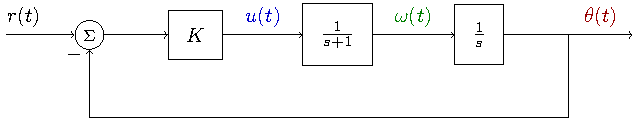
\includegraphics[width=1.0\linewidth]{../../figures/block-DC-feedback}
\end{center}
\end{column}

\begin{column}{0.5\columnwidth}
\begin{center}
 \def\ggain{1}
 \def\Tcnst{1}
 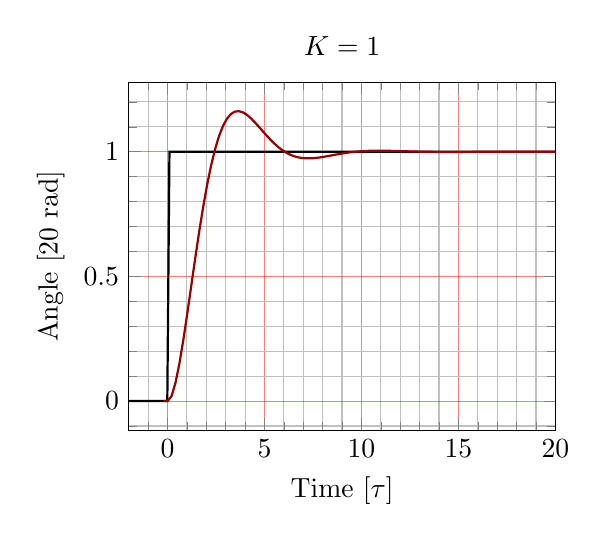
\begin{tikzpicture}
   \begin{axis}[
   width=7cm,
   height=6cm,
   grid = both,
   xlabel = {Time [$\tau$]},
   ylabel = {Angle [20 rad]},
   title = {$K=1$},
   %xtick = {0, \tdelay, \tone, \two},
   %xticklabels = {0, $\theta$, $\theta+\frac{\tau}{3}$, $\theta + \tau$},
   %ytick = {0, \yone, \ytwo, \uampl, \yfinal},
   %yticklabels = {0, $0.283y_{f}$, $0.632y_f$, $u_f$, $y_f$},
   xmin = -2, xmax=20,
   minor y tick num=4,
   minor x tick num=4,
   every major grid/.style={red, opacity=0.5},
   ]
     \addplot [thick, black, no marks, domain=-2:20, samples=200] {x>0};
     \addplot [thick, red!60!black, no marks, domain=-0.2:20, samples=100] {(x>0)*(1 - (exp(-x/2)* (sqrt(3)* cos(deg((sqrt(3)* x)/2)) + sin(deg((sqrt(3)* x)/2))))/sqrt(3))};
   \end{axis}
 \end{tikzpicture}
\end{center}
\end{column}
\end{columns}
\end{frame}


\begin{frame}[label={sec:orgd7e7bec}]{Proportional control of the normalized DC motor}
\begin{columns}
\begin{column}{0.5\columnwidth}
\begin{center}
 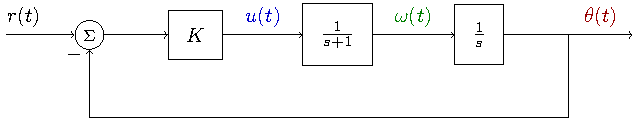
\includegraphics[width=1.0\linewidth]{../../figures/block-DC-feedback}
\end{center}
\end{column}

\begin{column}{0.5\columnwidth}
\begin{center}
 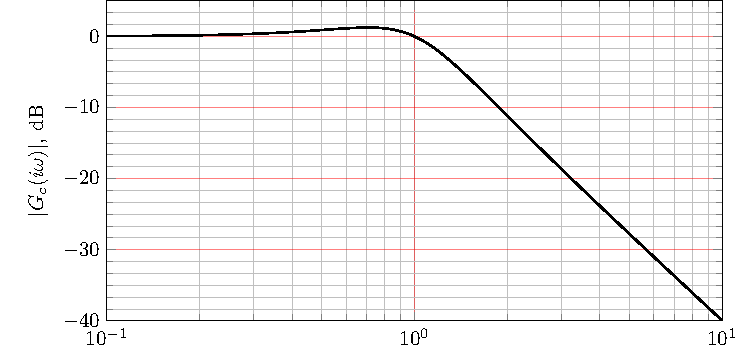
\includegraphics[width=1.0\linewidth]{../../figures/bode-closed-loop-normalized-DC}
\end{center}
\end{column}
\end{columns}
\end{frame}

\begin{frame}[label={sec:org116ddcb}]{Proportional control of the normalized DC motor}
\begin{columns}
\begin{column}{0.5\columnwidth}
\begin{center}
 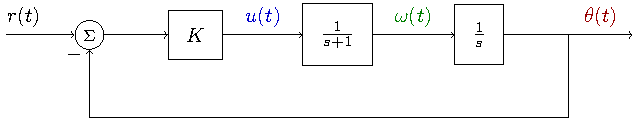
\includegraphics[width=1.0\linewidth]{../../figures/block-DC-feedback}
\end{center}

\alert{Activity} Determine the cross-over frequency and the phase margin.
\end{column}
\begin{column}{0.5\columnwidth}
\begin{center}
 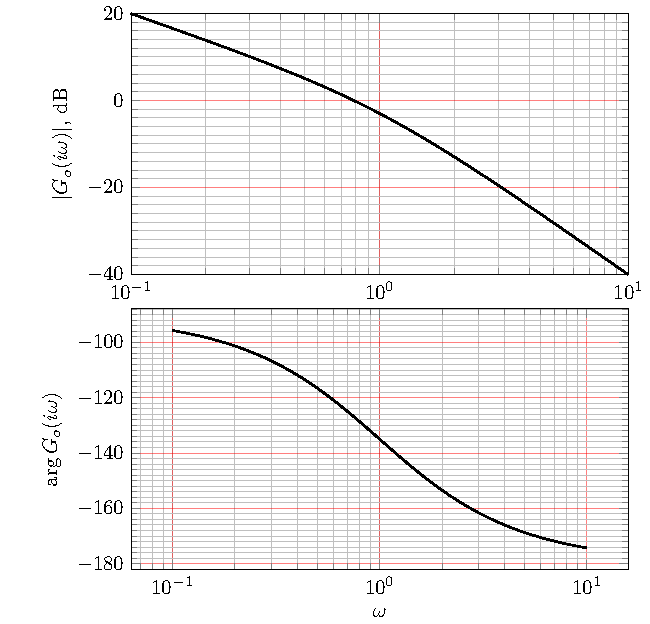
\includegraphics[width=1.0\linewidth]{../../figures/bode-loop-gain-normalized-DC}
\end{center}
\end{column}
\end{columns}
\end{frame}

\section{Lead-lag design}
\label{sec:org3f599d0}

\begin{frame}[label={sec:org248bcd9}]{Specifications on the frequency properties of the closed-loop system}
\begin{center}
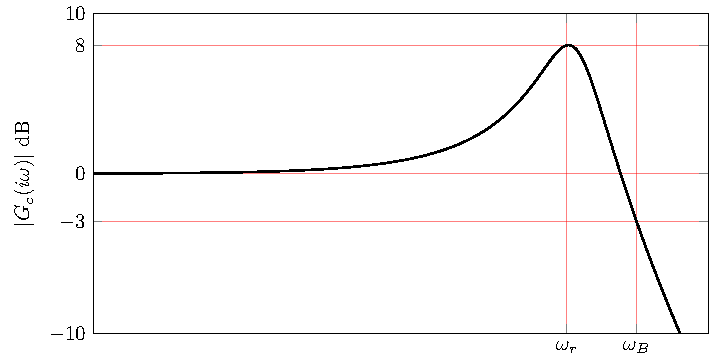
\includegraphics[width=0.999\linewidth]{../../figures/spec-bode-closed-loop-new}
\end{center}
\end{frame}

\begin{frame}[label={sec:orgfb02603}]{How to achieve the frequency-domain specifications}
\begin{columns}
\begin{column}{0.28\columnwidth}
\[G_c(i\omega) = \frac{ G_o(i\omega)}{1 + G_o(i\omega)}\]

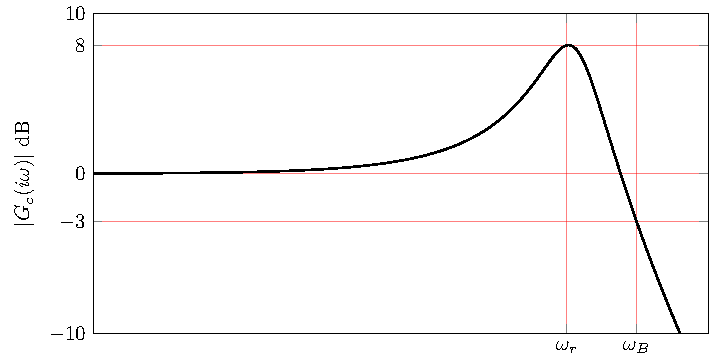
\includegraphics[width=1.1\linewidth]{../../figures/spec-bode-closed-loop-new}

\alert{Activity} Which of the Bode plots to the right shows the correct loop gain \(G_o(i\omega)\)?
\end{column}

\begin{column}{0.72\columnwidth}
\begin{center}
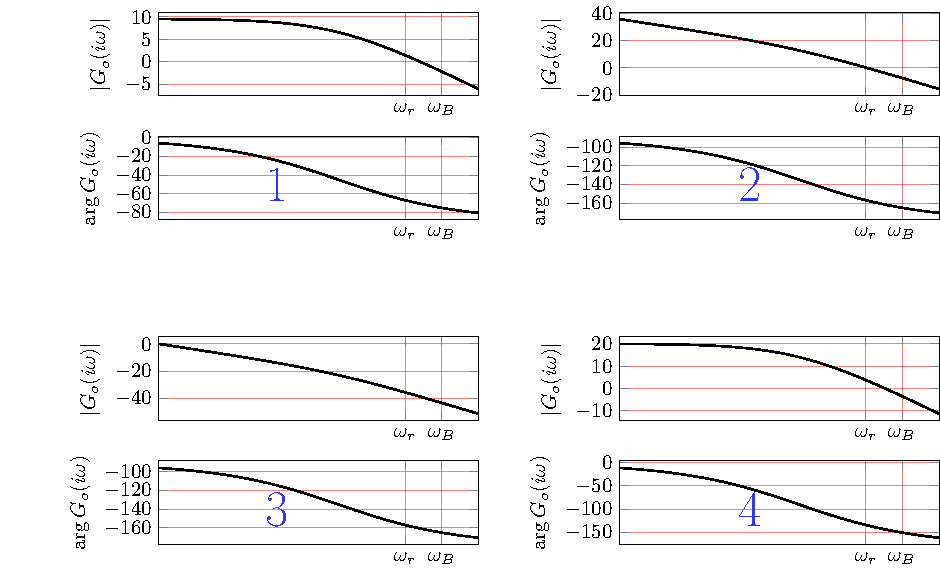
\includegraphics[width=1.02\linewidth]{../../figures/spec-bode-open-loop-new}
\end{center}
\end{column}
\end{columns}
\end{frame}

\begin{frame}[label={sec:orge229c60}]{From specifications on \(G_c\) to specifications on \(G_o\)}
\begin{center}
\begin{center}
\begin{tabular}{ll}
Closed-loop specifications & Loop gain specifications\\
\hline
High bandwidth \(\omega_B\) & High cross-over frequency \(\omega_c\)\\
Low resonance peak \(M_p\) & Large phase margin \(\varphi_m\)\\
Static gain \(G_c(0) \approx 1\) & static gain \(G_o(0)\) high\\
\hline
\end{tabular}
\end{center}
\end{center}
\end{frame}


\section{Design example - DC motor}
\label{sec:orgb95d5d4}
\begin{frame}[label={sec:orgde74340}]{Position control of the DC motor}
\begin{columns}
\begin{column}{0.7\columnwidth}
\begin{center}
  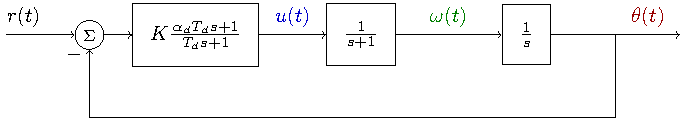
\includegraphics[width=0.9\linewidth]{../../figures/block-DC-lead-compensator}
\end{center}
\end{column}
\begin{column}{0.3\columnwidth}
Specifications:
\begin{enumerate}
\item \(\omega_B \approx \omega_c = \unit{2}{\rad\per\second}\)
\item \(\varphi_m > \unit{60}{\degree}\)
\end{enumerate}
\end{column}
\end{columns}
\end{frame}


\begin{frame}[label={sec:org4b1c81f}]{Position control of the DC motor}
\begin{columns}
\begin{column}{0.6\columnwidth}
\begin{center}
  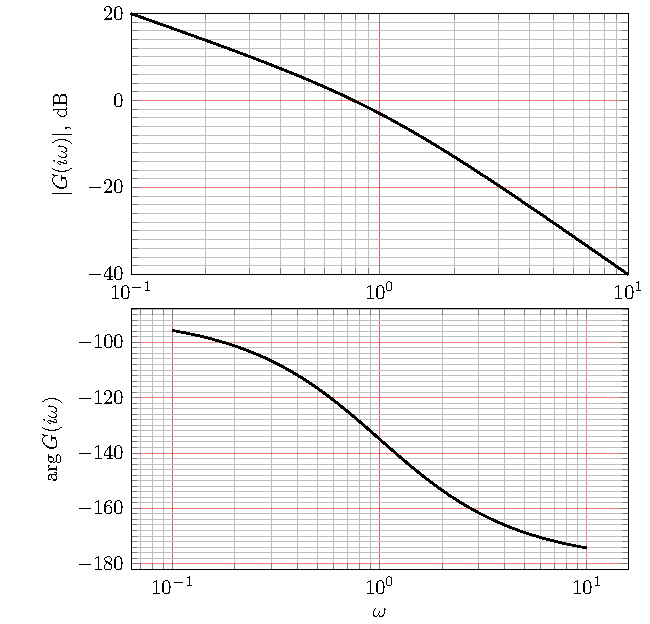
\includegraphics[width=0.9\linewidth]{../../figures/bode-plant-normalized-DC}
\end{center}
\end{column}

\begin{column}{0.4\columnwidth}
Specifications:
\begin{enumerate}
\item \(\omega_B \approx \omega_c = \unit{2}{\rad\per\second}\)
\item \(\varphi_m = \arg G_o(i\omega_c) - (-\unit{180}{\degree}) > \unit{60}{\degree}\)
\end{enumerate}


\alert{Activity}
\begin{enumerate}
\item What is \(|G (i\omega_c)|\)?
\item What is  \(\arg G(i\omega_c)\)?
\item What should \(\arg G_o(i\omega_c)\) be to satisfy the phase margin requirement?
\item How much phase advance is needed at the desired cross-over frequency?
\end{enumerate}
\end{column}
\end{columns}
\end{frame}

\begin{frame}[label={sec:org82d09fd}]{Position control of the DC motor - obtaining the phase advance}
\[F_{lead}(s) = \frac{\alpha_d T_d s + 1}{T_d s + 1}\]

\begin{center}
  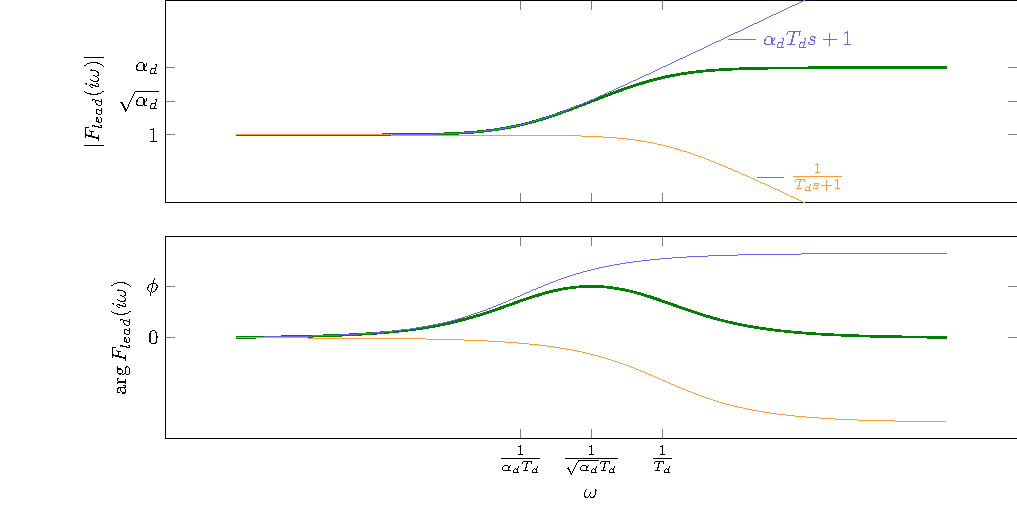
\includegraphics[width=0.9\linewidth]{../../figures/bode-lead-compensator}
\end{center}
\end{frame}

\begin{frame}[label={sec:org9e2f132}]{The maximum phase advance of the lead compensator}
\begin{columns}
\begin{column}{0.4\columnwidth}
\[F_{lead}(s) = \frac{\alpha_d T_d s + 1}{T_d s + 1}\]

\[ \phi = \max \arg F_{lead}(i\omega)\]
\[ \sin\phi = \frac{\alpha_d -1}{\alpha_d + 1}\quad \Leftrightarrow \quad \alpha_d = \frac{1 + \sin\phi}{1-\sin\phi} \]

\alert{Activity} Find the value of \(\alpha_d\) that gives the necessary maximum positive phase \(\arg F_{lead}(i\omega_c) = \unit{34}{\degree}\).
\end{column}


\begin{column}{0.6\columnwidth}
\begin{center}
  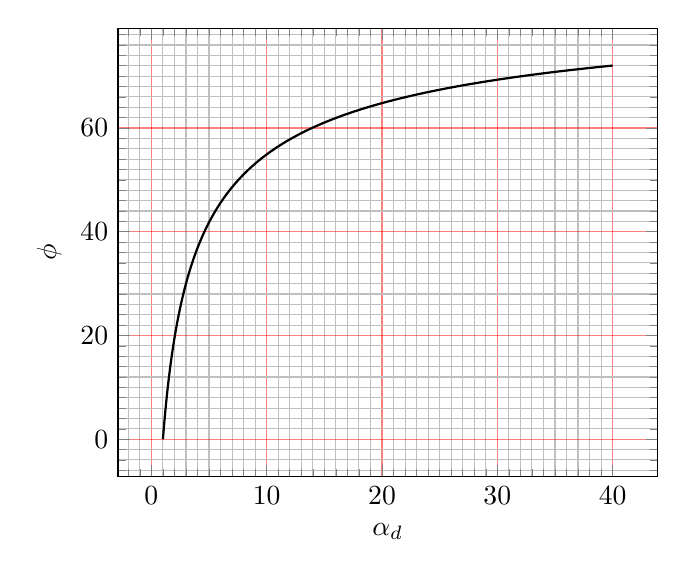
\begin{tikzpicture}
    \begin{axis}[xlabel=$\alpha_d$, ylabel=$\phi$,
    grid=both,
    minor x tick num=9,
    minor y tick num=9,
      every major grid/.style={red, opacity=0.5},
]
    \addplot[black, thick, smooth, no marks, domain=1:40, samples=300] {asin((\x-1)/(\x+1))};
    \end{axis}
  \end{tikzpicture}
\end{center}
\end{column}
\end{columns}
\end{frame}

\begin{frame}[label={sec:org776c929}]{Position control of the DC motor - placing the phase peak}
\[F_{lead}(s) = \frac{\alpha_d T_d s + 1}{T_d s + 1}\]

\begin{center}
  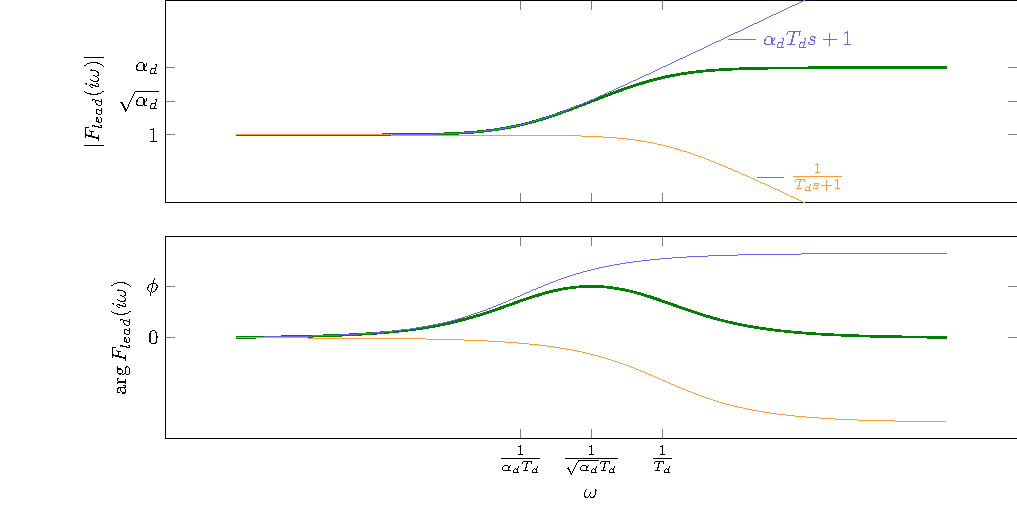
\includegraphics[width=0.9\linewidth]{../../figures/bode-lead-compensator}
\end{center}

\alert{Activity} Determine the time constant \(T_d\) that will place the peak of the phase curve at the desired cross-over frequency \(\omega_c = 2\).
\end{frame}


\begin{frame}[label={sec:org7a24b2c}]{Position control of the DC motor - The resulting lead compensator}
\[F_{lead}(s) = \frac{\alpha_d T_d s + 1}{T_d s + 1} = \frac{s + 1}{0.25s + 1}\]

\begin{center}
  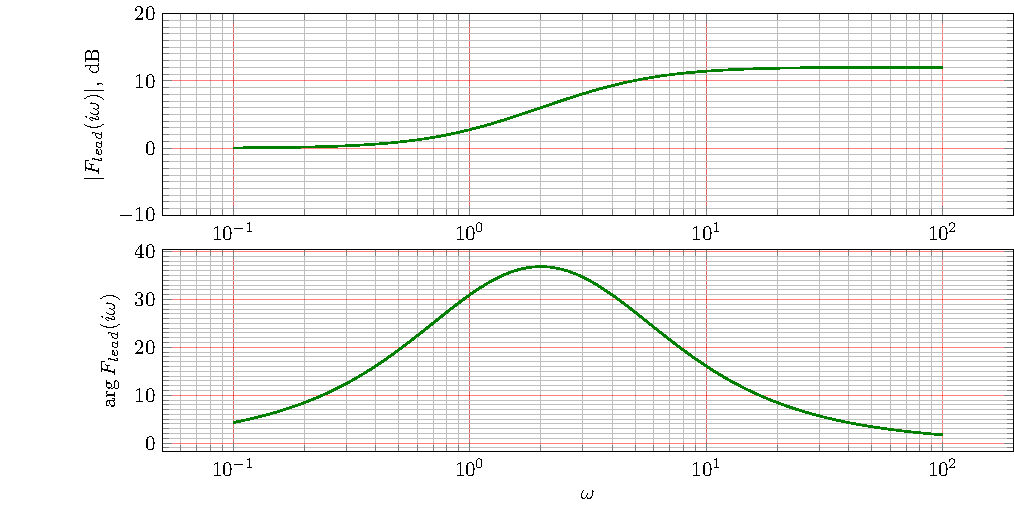
\includegraphics[width=0.9\linewidth]{../../figures/bode-lead-compensator-numerical}
\end{center}
\end{frame}


\begin{frame}[label={sec:orga5ebf8e}]{Position control of the DC motor - Getting the gain right}
\begin{columns}
\begin{column}{0.5\columnwidth}
\begin{center}
  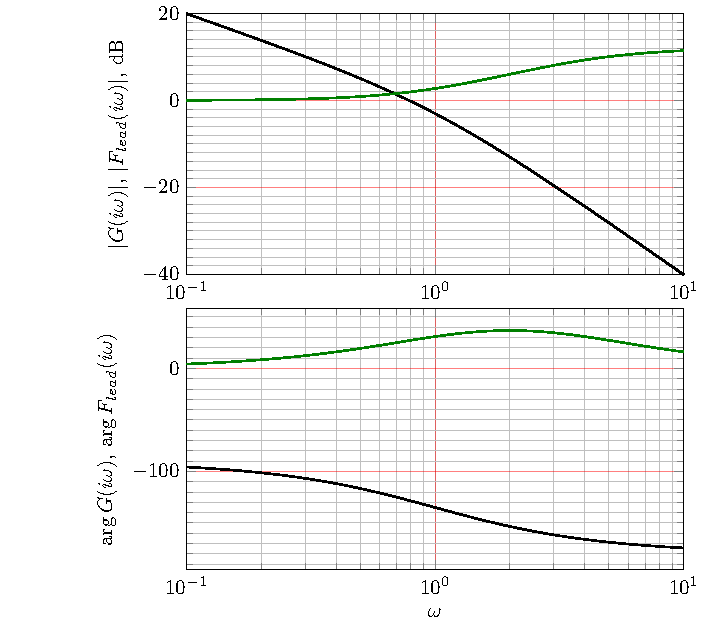
\includegraphics[width=1.0\linewidth]{../../figures/bode-plant-lead-normalized-DC}
\end{center}
\end{column}

\begin{column}{0.4\columnwidth}
Specifications

\begin{enumerate}
\item \(\omega_B =\approx \omega_c = \unit{2}{\rad\per\second}\)
\item \(\varphi_m = \arg G_o(i\omega_c) - (-\unit{180}{\degree}) > \unit{60}{\degree}\)
\end{enumerate}

\alert{Activity}
\begin{align*}
20\log G_o(i\omega) &= 20\log K F(i\omega)G(i\omega)\\
 &= 20\log K + 20\log F(i\omega) + 20\log G(i\omega)
 \end{align*}
so, what should the gain \(K\) be to obtain
\[  |G_o(i2)| = 1 = 0\text{dB}?\]
\end{column}
\end{columns}
\end{frame}


\begin{frame}[label={sec:orge3ebc31}]{Position control of the DC motor - Results}
\begin{columns}
\begin{column}{0.5\columnwidth}
\begin{center}
  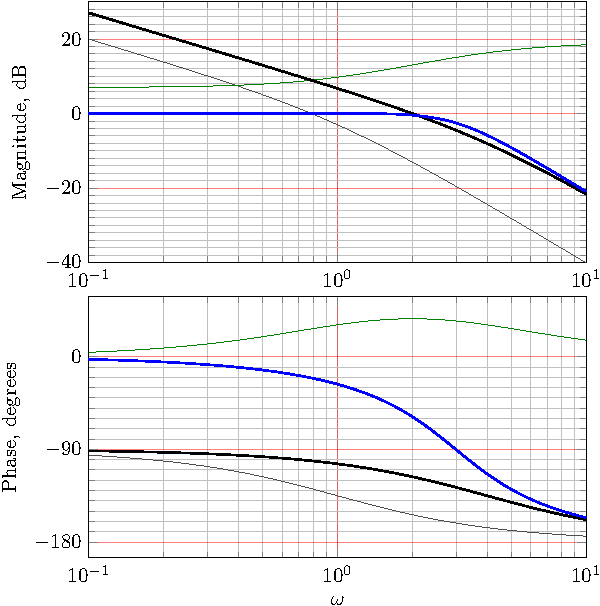
\includegraphics[width=1.0\linewidth]{../../figures/bode-loop-gain-lead-normalized-DC-crop}
\end{center}
\end{column}


\begin{column}{0.4\columnwidth}
\begin{center}
 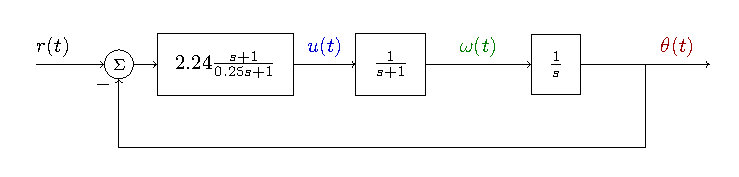
\includegraphics[width=1.0\linewidth]{../../figures/block-DC-lead-compensator-numerical}
\end{center}

\alert{Activity} Identify the frequency responses of: 1) The plant, 2) The compensator, 3) The loop gain, and 4) The closed-loop system.
\end{column}
\end{columns}
\end{frame}

\begin{frame}[label={sec:org7facc9c}]{Position control of the DC motor - Results}
\begin{columns}
\begin{column}{0.5\columnwidth}
\begin{center}
 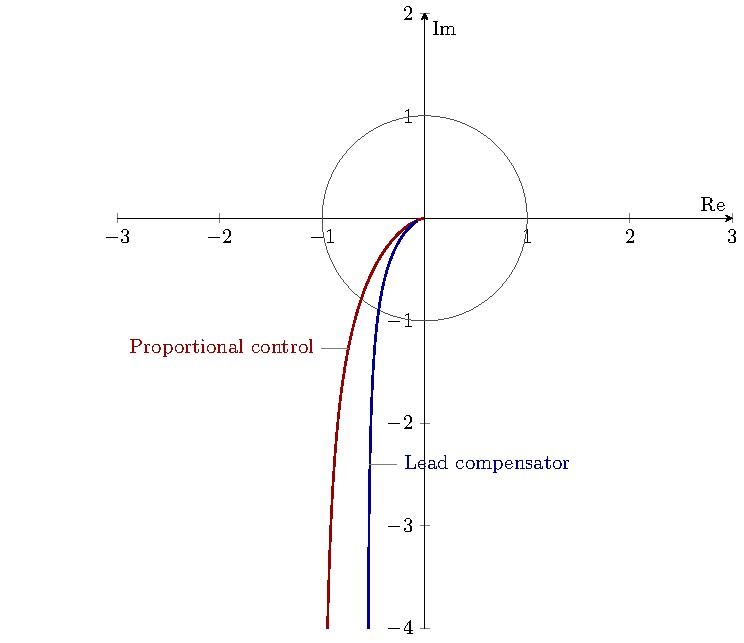
\includegraphics[width=\linewidth]{../../figures/nyquist-loop-gain-lead-normalized-DC}
\end{center}
\end{column}

\begin{column}{0.5\columnwidth}
    \begin{center}
  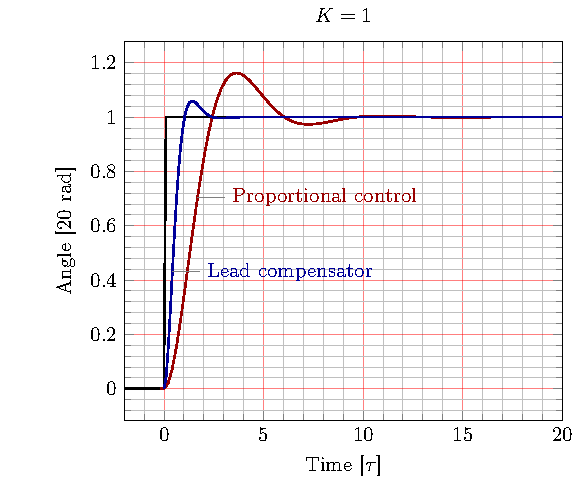
\includegraphics[width=1.0\linewidth]{../../figures/step-response-lead-normalized-DC}
\end{center}
\end{column}
\end{columns}
\end{frame}


\begin{frame}[label={sec:orgb3c5947}]{Applying the compensator design to a particular motor}
\begin{center}
 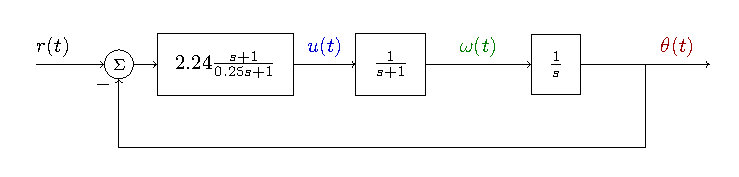
\includegraphics[width=.7\linewidth]{../../figures/block-DC-lead-compensator-numerical}
\end{center}

\pause
\begin{center}
 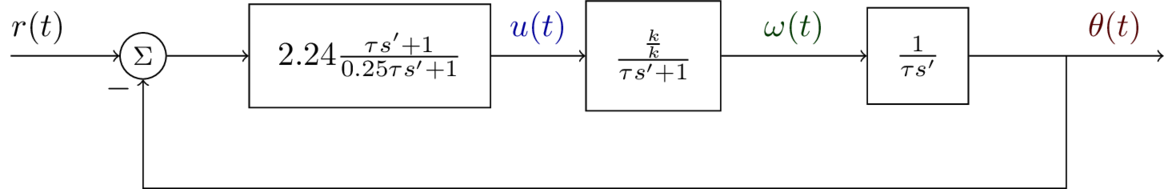
\includegraphics[width=.7\linewidth]{../../figures/block-DC-lead-compensator-particular-sol}
\end{center}

\pause
\begin{center}
 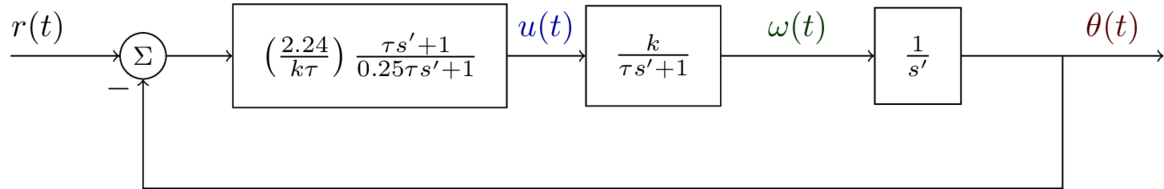
\includegraphics[width=.7\linewidth]{../../figures/block-DC-lead-compensator-particular-sol-white}
\end{center}
\end{frame}
\end{document}